To uncover latent relationships within multiple documents, we utilize Vicuna~\cite{vicuna2023} for knowledge graph completion. Vicuna is a cutting-edge model designed for natural language understanding tasks. Leveraging advanced techniques, it excels in tasks such as text summarization, sentiment analysis, and language translation. Its robust architecture ensures high-performance outcomes across diverse applications.

The process involves inputting multimodal multi-document claims generated by~\textbf{KG2Claim} into Vicuna. Subsequently, prompts are employed to extract latent information from these claims. This ensures the incorporation of latent information derived from such claims. Furthermore, the completion claims are inserted into knowledge graphs to enhance available resources.

\begin{figure}
\centering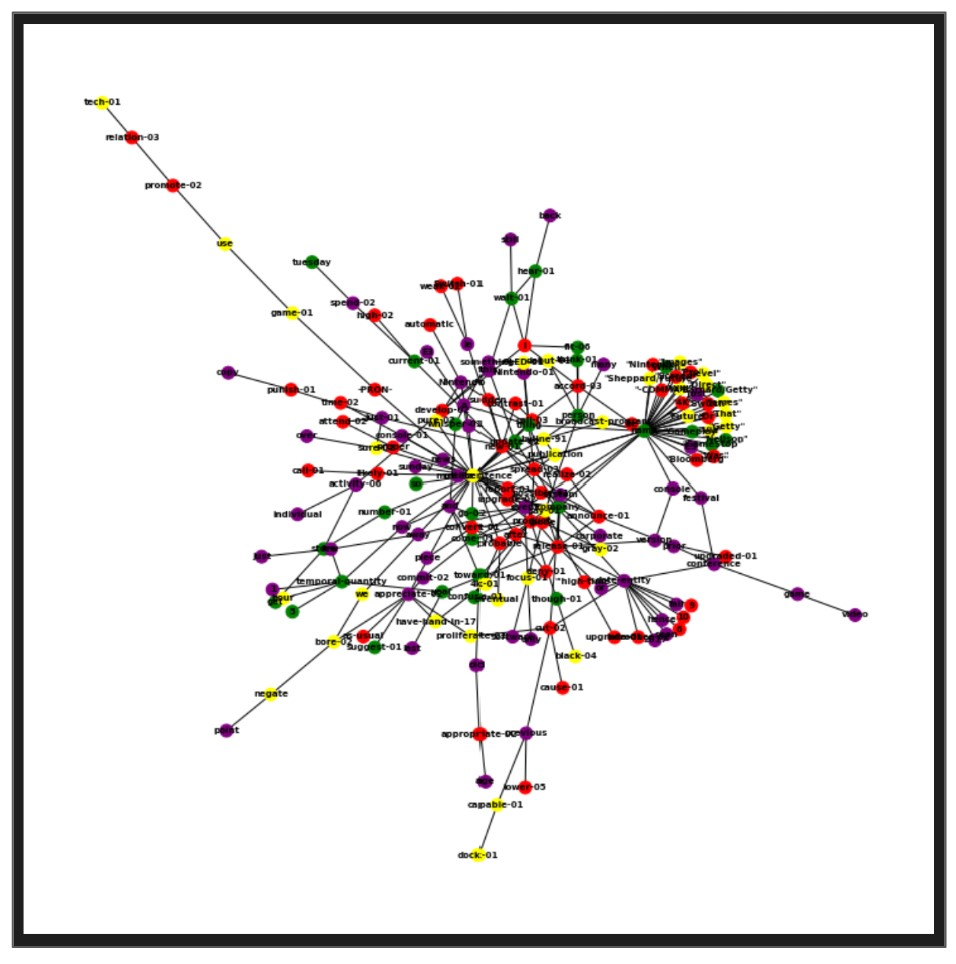
\includegraphics[width=\textwidth,height=\textwidth,keepaspectratio]{images/11.jpg}
  \caption{The knowledge graph is depicted with color-coded elements denoting multi-document sources. In our research, a maximum of four documents is utilized.}
  \label{fig:visulization}
\end{figure}